% ------------------------------------------------------------------------------
% TYPO3 Version 11.1 - What's New (English Version)
%
% @author	Michael Schams <schams.net>
% @license	Creative Commons BY-NC-SA 3.0
% @link		https://typo3.org/help/documentation/whats-new/
% @language	English
% ------------------------------------------------------------------------------
% .

\documentclass[t]{beamer}

% suppress navigation bar
\beamertemplatenavigationsymbolsempty

\mode<presentation>
{
	\usetheme{typo3slides}
}

% global variables
\title{TYPO3 Version 11.1 - What's New}
\subtitle{Summary of the new features, changes and improvements}
\author{
	\centerline{Created by:}
	\centerline{Michael Schams}
}

\date{\today}

\begin{document}

% select TYPO3 Share font
\sharefont

% ------------------------------------------------------------------------------
% Title Page
% ------------------------------------------------------------------------------

\begingroup
	\setbeamercolor{normal text}{fg=white,bg=typo3orange}
	\setbeamercolor{title}{fg=white}
	\setbeamercolor{author}{fg=white}
	\setbeamertemplate{footline}[default]
	\begin{frame}
		\titlepage
	\end{frame}
\endgroup

% ------------------------------------------------------------------------------
% Table of Contents
% ------------------------------------------------------------------------------

\section*{TYPO3 Version 11.1 - What's New}
\begin{frame}[fragile]
	\frametitle{Chapter Overview}
	\framesubtitle{Chapter Overview}

	\tableofcontents

\end{frame}

% ------------------------------------------------------------------------------

% Chapter "Introduction"
% ------------------------------------------------------------------------------
% TYPO3 Version 11.1 - What's New (Italian Version)
%
% @license	Creative Commons BY-NC-SA 3.0
% @link		http://typo3.org/download/release-notes/whats-new/
% @language	Italian
% ------------------------------------------------------------------------------

\section{Extbase and Fluid}
\begin{frame}[fragile]
	\frametitle{Extbase and Fluid}

	\begin{center}\huge{Chapter 3:}\end{center}
	\begin{center}\huge{\color{typo3darkgrey}\textbf{Extbase and Fluid}}\end{center}

\end{frame}

% ------------------------------------------------------------------------------

% ------------------------------------------------------------------------------
% TYPO3 Version 11.1 - What's New (German Version)
%
% @license	Creative Commons BY-NC-SA 3.0
% @link		https://typo3.org/help/documentation/whats-new/
% @language	German
% ------------------------------------------------------------------------------
% TYPO3 Version 11.1 - The Facts

\begin{frame}[fragile]
	\frametitle{Introduction}
	\framesubtitle{TYPO3 Version 11.1 - The Facts}

	\begin{itemize}
		\item Release date: 23 February 2021
		\item Release type: Sprint Release
	\end{itemize}

	\begin{figure}
		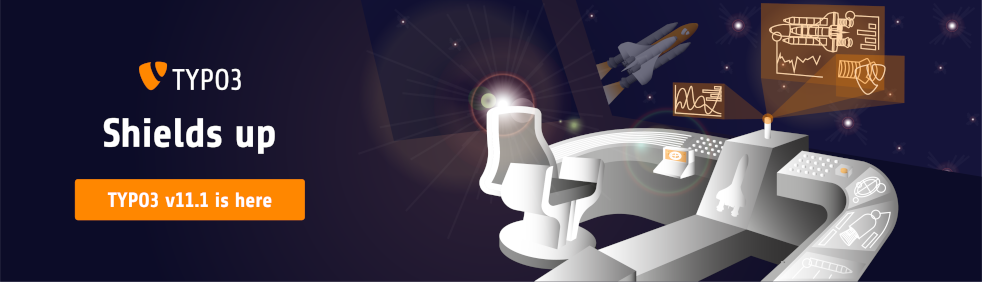
\includegraphics[width=0.95\linewidth]{Introduction/typo3-v11-1-banner.png}
	\end{figure}

\end{frame}

% ------------------------------------------------------------------------------

% ------------------------------------------------------------------------------
% TYPO3 Version 11.1 - What's New (English Version)
%
% @author	Michael Schams <schams.net>
% @license	Creative Commons BY-NC-SA 3.0
% @link		https://typo3.org/help/documentation/whats-new/
% @language	English
% ------------------------------------------------------------------------------
% TYPO3 Version 11.1 - Executive Summary

\begin{frame}[fragile]
	\frametitle{Introduction}
	\framesubtitle{Executive Summary}

	\small
		We are pleased to announce TYPO3 version 11.1, with multi-factor
		authentication built into the TYPO3 Core and some great usability
		improvements of the backend user interface.

		\vspace{0.2cm}

		Perfectly in time and equipped with all features as promised, TYPO3
		version 11.1 marks another milestone on our route towards the LTS
		(long-term support) release later this year.

		\vspace{0.2cm}

		The system requirements for TYPO3 v11.1 remain the same as for v11.0.
		The same applies to our support and maintenance promise.

	\normalsize

\end{frame}

% ------------------------------------------------------------------------------

% ------------------------------------------------------------------------------
% TYPO3 Version 11.1 - What's New (English Version)
%
% @author	Michael Schams <schams.net>
% @license	Creative Commons BY-NC-SA 3.0
% @link		https://typo3.org/help/documentation/whats-new/
% @language	English
% ------------------------------------------------------------------------------
% System Requirements

\begin{frame}[fragile]
	\frametitle{Introduction}
	\framesubtitle{System Requirements}

	\begin{itemize}
		\item PHP version 7.4+
		\item PHP settings:

			\begin{itemize}
				\item \texttt{memory\_limit} >= 256M
				\item \texttt{max\_execution\_time} >= 240s
				\item \texttt{max\_input\_vars} >= 1500
				\item compilation option \texttt{-}\texttt{-disable-ipv6} must \underline{not} be used
			\end{itemize}

		\item Most database servers supported by \textbf{Doctrine DBAL} also work with TYPO3.
			Tested DB engines are for example:
	\end{itemize}

	\begin{figure}
		
\includegraphics[width=0.80\linewidth]{Introduction/logo-databases.png}
	\end{figure}

\end{frame}

% ------------------------------------------------------------------------------

% ------------------------------------------------------------------------------
% TYPO3 Version 11.1 - What's New (Italian Version)
%
% @license	Creative Commons BY-NC-SA 3.0
% @link		https://typo3.org/help/documentation/whats-new/
% @language	Italian
% ------------------------------------------------------------------------------
% Development, Support, and Maintenance Timeline

\begin{frame}[fragile]
	\frametitle{Introduction}
	\framesubtitle{Development, Support, and Maintenance Timeline}

	\textbf{TYPO3 v11}

	\begin{figure}
		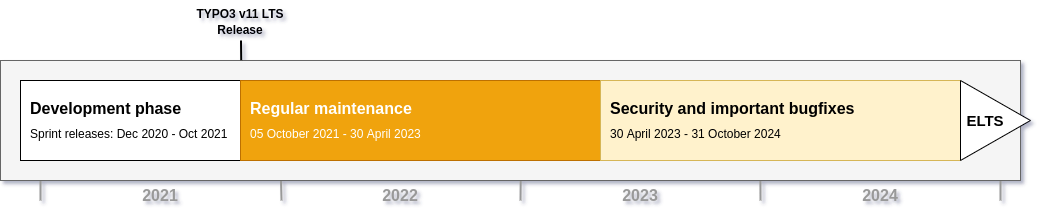
\includegraphics[width=1\linewidth]{Introduction/typo3-v11-lifecycle.png}
	\end{figure}

	\textbf{Extended long-term support (ELTS)}\newline
	\smaller
		The \href{https://typo3.com}{TYPO3 GmbH} offers further support options
		for TYPO3 v11 LTS even after 31 October 2024 for up to two additional
		years.
	\normalsize

\end{frame}

% ------------------------------------------------------------------------------

% ------------------------------------------------------------------------------
% TYPO3 Version 11.1 - What's New (Dutch Version)
%
% @license	Creative Commons BY-NC-SA 3.0
% @link		https://typo3.org/help/documentation/whats-new/
% @language	Dutch
% ------------------------------------------------------------------------------
% TYPO3 v11 Release Dates

\begin{frame}[fragile]
	\frametitle{Introduction}
	\framesubtitle{TYPO3 v11 Release Dates}

	Planned release dates and their primary focus:

	\begin{itemize}
		\item v11.0 \tabto{1.1cm}22/Dec/2020\tabto{3.4cm}New system requirements and breaking changes
		\item
			\begingroup
				\color{typo3orange}
				v11.1 \tabto{1.1cm}23/Feb/2021\tabto{3.4cm}Multi-factor authentication
			\endgroup
		\item v11.2 \tabto{1.1cm}04/May/2021\tabto{3.4cm}Link sharing for TYPO3 Backend
		\item v11.3 \tabto{1.1cm}13/Jul/2021\tabto{3.4cm}(\textit{to be determined})
		\item v11.4 \tabto{1.1cm}07/Sep/2021\tabto{3.4cm}Feature freeze
		\item v11.5 \tabto{1.1cm}05/Oct/2021\tabto{3.4cm}LTS Release (Long-term Support)

	\end{itemize}

	\smaller
		\url{https://typo3.org/cms/roadmap}\newline
		\url{https://typo3.org/article/a-first-glimpse-of-typo3-v11}
	\normalsize

\end{frame}

% ------------------------------------------------------------------------------

% ------------------------------------------------------------------------------
% TYPO3 Version 11.1 - What's New (Dutch Version)
%
% @license	Creative Commons BY-NC-SA 3.0
% @link		https://typo3.org/help/documentation/whats-new/
% @language	Dutch
% ------------------------------------------------------------------------------
% Installation

\begin{frame}[fragile]
	\frametitle{Introduction}
	\framesubtitle{Installation}

	% decrease font size for code listing
	\lstset{basicstyle=\fontsize{8}{10}\ttfamily}

	\begin{itemize}
		\item Official \textit{classic} installation procedure under Linux/Mac OS X\newline
			(DocumentRoot for example \texttt{/var/www/site/htdocs}):
\begin{lstlisting}
$ cd /var/www/site
$ wget --content-disposition get.typo3.org/11.1
$ tar xzf typo3_src-11.1.0.tar.gz
$ cd htdocs
$ ln -s ../typo3_src-11.1.0 typo3_src
$ ln -s typo3_src/index.php
$ ln -s typo3_src/typo3
$ touch FIRST_INSTALL
\end{lstlisting}

		\item See \href{https://docs.typo3.org/m/typo3/guide-installation/master/en-us/}{Installation and Upgrade Guide}
			for details about Microsoft Windows systems.

	\end{itemize}
\end{frame}

% ------------------------------------------------------------------------------

% ------------------------------------------------------------------------------
% TYPO3 Version 11.1 - What's New (Serbian Version)
%
% @license	Creative Commons BY-NC-SA 3.0
% @link		https://typo3.org/help/documentation/whats-new/
% @language	Serbian
% ------------------------------------------------------------------------------
% Installation using Composer

\begin{frame}[fragile]
	\frametitle{Installation and Upgrade}
	\framesubtitle{Installation Using \texttt{Composer}}

	% decrease font size for code listing
	\lstset{basicstyle=\fontsize{8}{10}\ttfamily}

	\begin{itemize}
		\item Installation using \href{https://getcomposer.org}{PHP Composer} under Linux, macOS, and Windows 10:
\begin{lstlisting}
$ cd /var/www/site/
$ composer create-project typo3/cms-base-distribution:^11 typo3v11
\end{lstlisting}

		\item Alternatively, create your custom \texttt{composer.json} file and run:
\begin{lstlisting}
$ composer install
\end{lstlisting}

		\item The \href{https://get.typo3.org/misc/composer/helper}{Composer Helper}
			online tool makes package selection easy.

		\item Further details are available in the
			\href{https://docs.typo3.org/m/typo3/guide-installation/master/en-us/}{Installation and Upgrade Guide}.

	\end{itemize}
\end{frame}

% ------------------------------------------------------------------------------


% Chapter "Backend User Interface"
% ------------------------------------------------------------------------------
% TYPO3 Version 11.1 - What's New (Italian Version)
%
% @license	Creative Commons BY-NC-SA 3.0
% @link		http://typo3.org/download/release-notes/whats-new/
% @language	Italian
% ------------------------------------------------------------------------------

\section{Extbase and Fluid}
\begin{frame}[fragile]
	\frametitle{Extbase and Fluid}

	\begin{center}\huge{Chapter 3:}\end{center}
	\begin{center}\huge{\color{typo3darkgrey}\textbf{Extbase and Fluid}}\end{center}

\end{frame}

% ------------------------------------------------------------------------------

% ------------------------------------------------------------------------------
% TYPO3 Version 11.1 - What's New (Spanish Version)
%
% @license	Creative Commons BY-NC-SA 3.0
% @link		http://typo3.org/download/release-notes/whats-new/
% @language	Spanish
% ------------------------------------------------------------------------------
% Feature | 93117 | Add reset button to Backend User module filter

\begin{frame}[fragile]
	\frametitle{Backend User Interface}
	\framesubtitle{Reset Backend User Filter}

	The module "Backend Users" features a button to reset the user filter now.

	\begin{figure}
		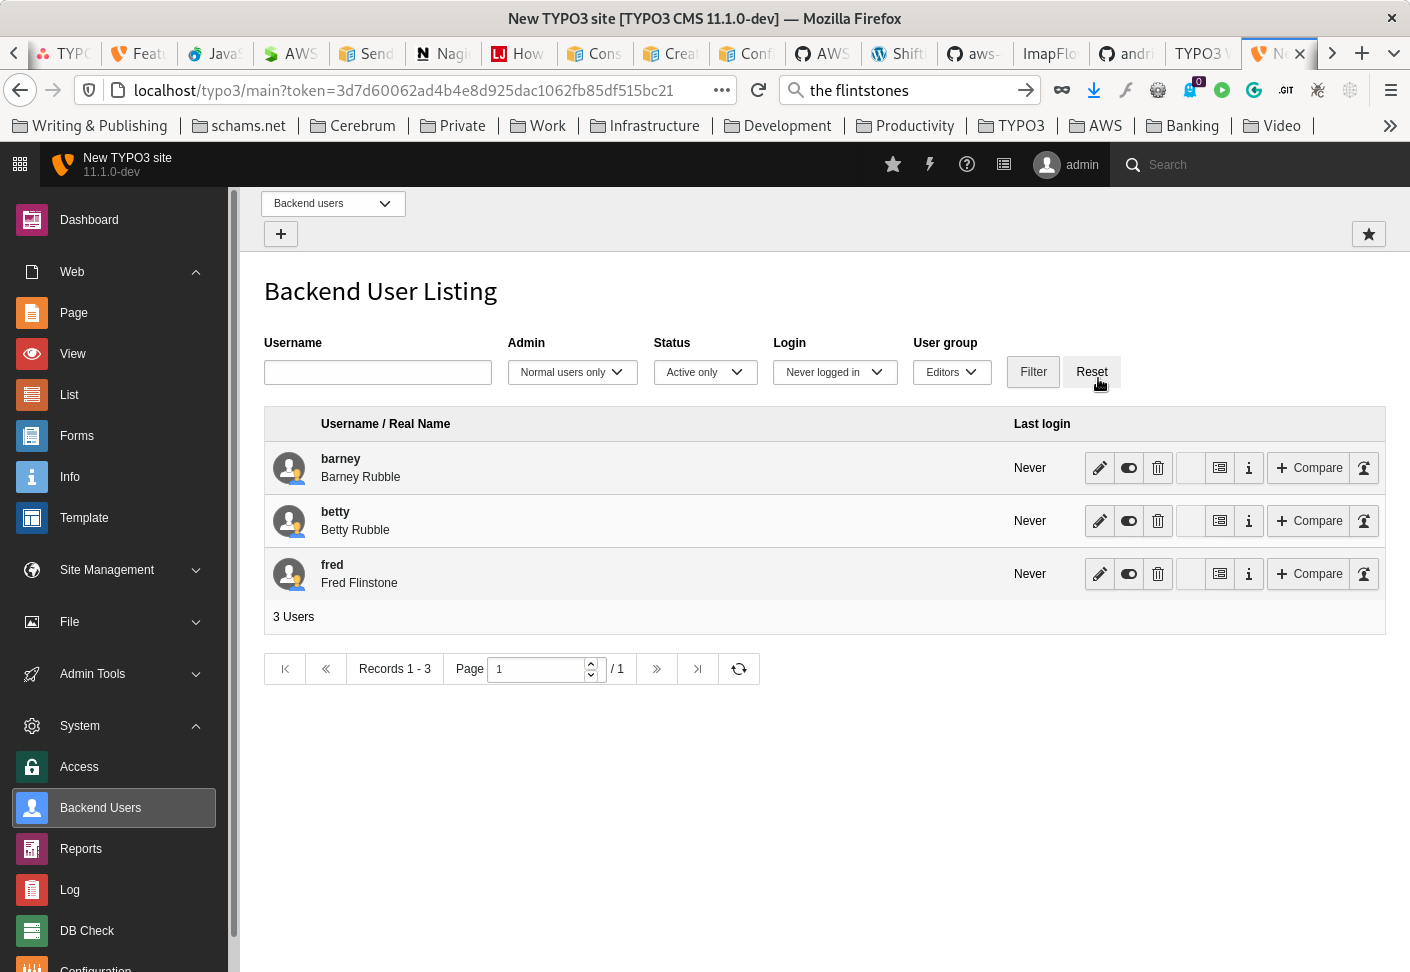
\includegraphics[width=0.9\linewidth]{BackendUserInterface/1612763310-ResetBackendUserModuleFilter.png}
	\end{figure}

\end{frame}

% ------------------------------------------------------------------------------

% ------------------------------------------------------------------------------
% TYPO3 Version 11.1 - What's New (Dutch Version)
%
% @license	Creative Commons BY-NC-SA 3.0
% @link		http://typo3.org/download/release-notes/whats-new/
% @language	Dutch
% ------------------------------------------------------------------------------
% Feature | 78760 | Resizable Navigation Component

\begin{frame}[fragile]
	\frametitle{Backend User Interface}
	\framesubtitle{Resizable Navigation Component}

	Backend users can now resize the \textit{navigation area} such as the pagetree
	component and file list. The icon to collapse/re-open has been moved inside
	the area.

	\begin{figure}
		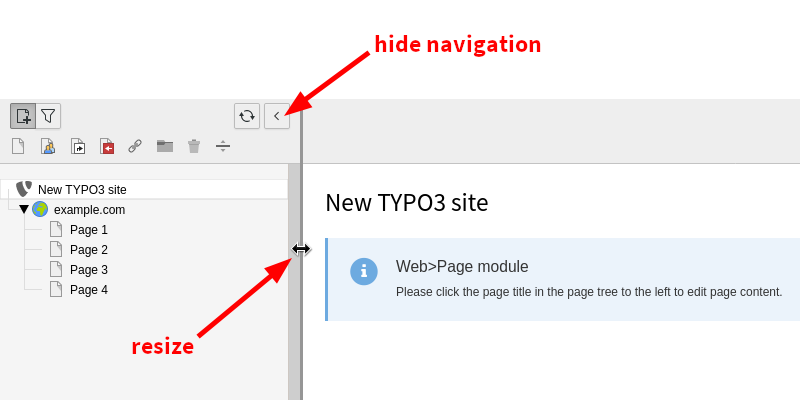
\includegraphics[width=0.75\linewidth]{BackendUserInterface/1612764665-ResizableNavigationComponent3.png}
	\end{figure}

\end{frame}

% ------------------------------------------------------------------------------

% ------------------------------------------------------------------------------
% TYPO3 Version 11.1 - What's New (English Version)
%
% @author	Michael Schams <schams.net>
% @license	Creative Commons BY-NC-SA 3.0
% @link		http://typo3.org/download/release-notes/whats-new/
% @language	English
% ------------------------------------------------------------------------------
% Feature | 92704 | Improve keyboard navigation for module menus

\begin{frame}[fragile]
	\frametitle{Backend User Interface}
	\framesubtitle{Backend Module Menus}

	Following the ARIA Best Practices 1.1, backend users can now navigate through
	the main module and the help menu by using the keyboard. This is ideal for
	users of screen readers or other assistive technology.

%	\begin{figure}
%		\includegraphics[width=0.9\linewidth]{BackendUserInterface/1613179329-BackendModuleMenusAccessibility.png}
%	\end{figure}

\end{frame}

% ------------------------------------------------------------------------------

% ------------------------------------------------------------------------------
% TYPO3 Version 11.1 - What's New (English Version)
%
% @author	Michael Schams <schams.net>
% @license	Creative Commons BY-NC-SA 3.0
% @link		http://typo3.org/download/release-notes/whats-new/
% @language	English
% ------------------------------------------------------------------------------
% ???

\begin{frame}[fragile]
	\frametitle{Backend User Interface}
	\framesubtitle{Filelist: Folder Tree}

	The "Filelist" received a visual overhaul and now uses the same lightweight
	SVG solution as the page tree does.

	\begin{figure}
		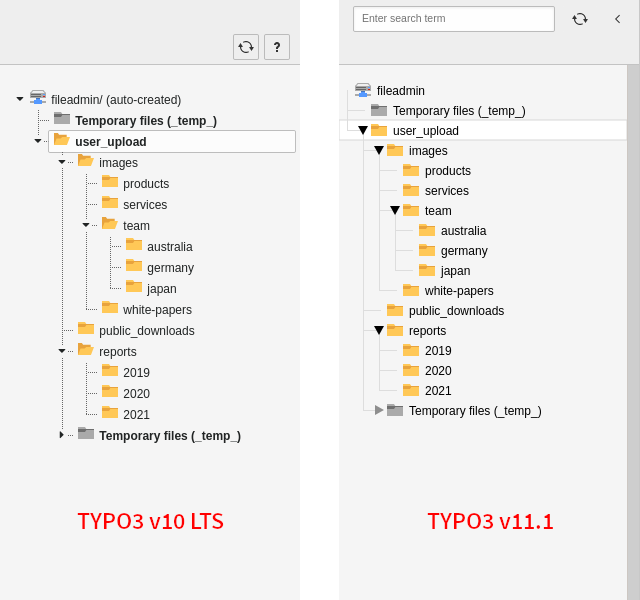
\includegraphics[width=0.55\linewidth]{BackendUserInterface/1613729428-BackendModuleFilelist.png}
	\end{figure}

\end{frame}

% ------------------------------------------------------------------------------

% ------------------------------------------------------------------------------
% TYPO3 Version 11.1 - What's New (Serbian Version)
%
% @license	Creative Commons BY-NC-SA 3.0
% @link		http://typo3.org/download/release-notes/whats-new/
% @language	Serbian
% ------------------------------------------------------------------------------
% Feature | 93526 | Multi-Factor Authentication

\begin{frame}[fragile]
	\frametitle{Backend User Interface}
	\framesubtitle{Multi-factor Authentication}

	If activated, backend users can now add a second authentication factor to
	their login process (for example a time-based one-time password).

	\begin{figure}
		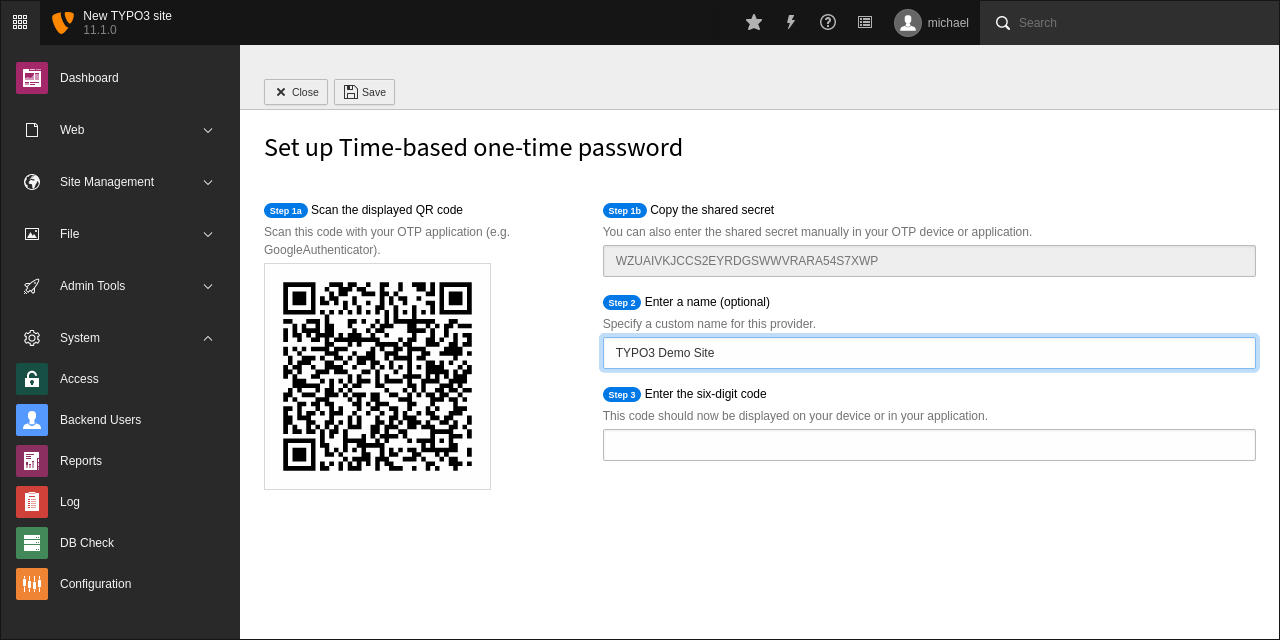
\includegraphics[width=0.8\linewidth]{BackendUserInterface/1613731375-BackendMfaSetup.png}
	\end{figure}

\end{frame}

% ------------------------------------------------------------------------------


% Chapter "Changes for Integrators and Developers"
% ------------------------------------------------------------------------------
% TYPO3 Version 11.1 - What's New (Italian Version)
%
% @license	Creative Commons BY-NC-SA 3.0
% @link		http://typo3.org/download/release-notes/whats-new/
% @language	Italian
% ------------------------------------------------------------------------------

\section{Extbase and Fluid}
\begin{frame}[fragile]
	\frametitle{Extbase and Fluid}

	\begin{center}\huge{Chapter 3:}\end{center}
	\begin{center}\huge{\color{typo3darkgrey}\textbf{Extbase and Fluid}}\end{center}

\end{frame}

% ------------------------------------------------------------------------------

% ------------------------------------------------------------------------------
% TYPO3 Version 11.1 - What's New (Italian Version)
%
% @license	Creative Commons BY-NC-SA 3.0
% @link		http://typo3.org/download/release-notes/whats-new/
% @language	Italian
% ------------------------------------------------------------------------------
% Feature | 93174 | Lazy console command list

\begin{frame}[fragile]
	\frametitle{Changes for Integrators and Developers}
	\framesubtitle{Console Command List (1)}

	\begin{itemize}
		\item The TYPO3 command line utility does not instantiate all available
			console commands anymore when a user executes \texttt{typo3 list}.
		\item This prevents the CLI tool from slowing down or breaking the
			command list (e.g.\ if a command is not instantiable).
		\item TYPO3 integrators benefit from a faster and more robust command list.
	\end{itemize}

\end{frame}

% ------------------------------------------------------------------------------

% ------------------------------------------------------------------------------
% TYPO3 Version 11.1 - What's New (French Version)
%
% @license	Creative Commons BY-NC-SA 3.0
% @link		http://typo3.org/download/release-notes/whats-new/
% @language	French
% ------------------------------------------------------------------------------
% Feature | 93174 | Lazy console command list

\begin{frame}[fragile]
	\frametitle{Changements pour les intégrateurs et développeurs}
	\framesubtitle{Console Command List (2)}

	\lstset{basicstyle=\fontsize{6}{8}\ttfamily}

	\begin{itemize}
		\item Two new properties have been added to the \texttt{console.command}
			dependency injection tag (to used in the \texttt{Services.yaml} file):
			\begin{itemize}
				\item \texttt{description}
				\item \texttt{hidden}
			\end{itemize}
			\vspace{0.2cm}
		\item The description must be set next to the command name:
\begin{lstlisting}
services:
  My\Namespace\Command\ExampleCommand:
    tags:
      - name: 'console.command'
        command: 'my:example'
        description: 'An example command that demonstrates some stuff'
        hidden: false
\end{lstlisting}

		\item Extension authors should use this method instead of setting
			description through \texttt{\$this->setDescription()}.

	\end{itemize}

\end{frame}

% ------------------------------------------------------------------------------

% ------------------------------------------------------------------------------
% TYPO3 Version 11.1 - What's New (Spanish Version)
%
% @license	Creative Commons BY-NC-SA 3.0
% @link		http://typo3.org/download/release-notes/whats-new/
% @language	Spanish
% ------------------------------------------------------------------------------
% Feature | 92942 | Allow icon overlay for newContentElementWizard elements

\begin{frame}[fragile]
	\frametitle{Changes for Integrators and Developers}
	\framesubtitle{Content Element Wizard}

	\lstset{basicstyle=\fontsize{6}{8}\ttfamily}

	\begin{itemize}
		\item New "new content element" wizard now supports an icon overlay for
			each wizard element.
		\item Useful for custom content elements that use the same
			\texttt{iconIdentifier} multiple times.
		\item For example (TSconfig):
\begin{lstlisting}
mod.wizards.newContentElement.wizardItems {
  common.elements {
    my_element {
      iconIdentifier = content-my-icon
      iconOverlay = content-my-icon-overlay
      title = LLL:EXT:my_extension/Resources/Private/Language/ContentTypes.xlf:title
      description = LLL:EXT:my_extension/Resources/Private/Language/ContentTypes.xlf:description
      tt_content_defValues {
        CType = my_element
      }
    }
  }
}
\end{lstlisting}

	\end{itemize}

\end{frame}

% ------------------------------------------------------------------------------

% ------------------------------------------------------------------------------
% TYPO3 Version 11.1 - What's New (Dutch Version)
%
% @license	Creative Commons BY-NC-SA 3.0
% @link		http://typo3.org/download/release-notes/whats-new/
% @language	Dutch
% ------------------------------------------------------------------------------
% Feature | 93455 | Backend Routes restricted to specified HTTP methods

\begin{frame}[fragile]
	\frametitle{Changes for Integrators and Developers}
	\framesubtitle{Backend Routes}

	\lstset{basicstyle=\fontsize{6}{8}\ttfamily}

	\begin{itemize}
		\item Backend routes can now be restricted to HTTP methods.\newline
			\small(e.g. \texttt{GET}, \texttt{POST}, \texttt{PUT}, \texttt{DELETE})
		\item The optional property "\texttt{methods}" can be set in the files:
			\begin{itemize}\smaller
				\item \texttt{Configuration/Backend/Routes.php}
				\item \texttt{Configuration/Backend/Ajax.php}
			\end{itemize}
			\vspace{0.2cm}
		\item For example:
\begin{lstlisting}
return [
  'my_route' => [
    'path' => '/benni/my-route',
    'methods' => ['POST'],
    'target' => MyVendor\MyPackage\Controller\MyRouteController::class . '::submitAction'
  ]
];
\end{lstlisting}

		\item No restriction applies if no property is set.

	\end{itemize}

\end{frame}

% ------------------------------------------------------------------------------

% ------------------------------------------------------------------------------
% TYPO3 Version 11.1 - What's New (English Version)
%
% @author	Michael Schams <schams.net>
% @license	Creative Commons BY-NC-SA 3.0
% @link		http://typo3.org/download/release-notes/whats-new/
% @language	English
% ------------------------------------------------------------------------------
% Feature | 92628 | Add Alt-Text To Login Logo
% Deprecation | 92628 | Login Logo without Alt-Text

\begin{frame}[fragile]
	\frametitle{Changes for Integrators and Developers}
	\framesubtitle{Backend Login Image}

	\lstset{basicstyle=\fontsize{6}{8}\ttfamily}

	\begin{itemize}
		\item The backend login image now supports an \texttt{alt}-tag.
		\item Without a value set, custom images produce a deprecation warning.
	\end{itemize}

	\begin{figure}
		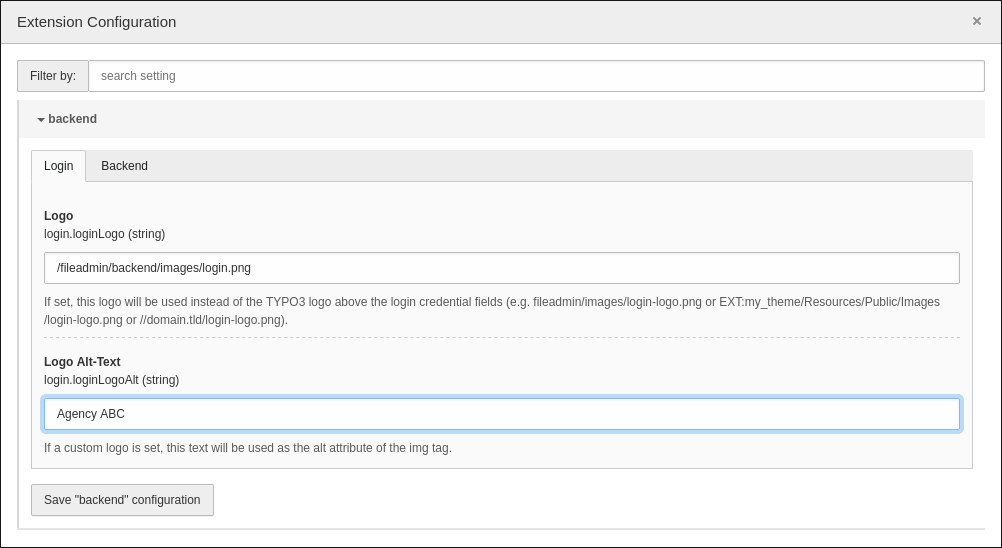
\includegraphics[width=0.75\linewidth]{ChangesForIntegratorsAndDevelopers/1613194504-BackendLoginLogoAlt.png}
	\end{figure}

\end{frame}

% ------------------------------------------------------------------------------

% ------------------------------------------------------------------------------
% TYPO3 Version 11.1 - What's New (French Version)
%
% @license	Creative Commons BY-NC-SA 3.0
% @link		http://typo3.org/download/release-notes/whats-new/
% @language	French
% ------------------------------------------------------------------------------
% Feature | 89509 | Data Processor to resolve FlexForm data

\begin{frame}[fragile]
	\frametitle{Changes for Integrators and Developers}
	\framesubtitle{FlexForm Data Processor}

	\lstset{basicstyle=\fontsize{6}{8}\ttfamily}

	\begin{itemize}
		\item A new data processor has been introduced:\newline
			\small\texttt{TYPO3\textbackslash
				CMS\textbackslash
				Frontend\textbackslash
				DataProcessing\textbackslash
				FlexFormProcessor}\normalsize
		\item This makes FlexForms available in Fluid templates.
		\item For example (TypoScript):
\begin{lstlisting}
10 = TYPO3\CMS\Frontend\DataProcessing\FlexFormProcessor
10 {
  fieldName = my_flexform_field
  as = myOutputVariable
}
\end{lstlisting}

	\end{itemize}

\end{frame}

% ------------------------------------------------------------------------------

% ------------------------------------------------------------------------------
% TYPO3 Version 11.1 - What's New (German Version)
%
% @license	Creative Commons BY-NC-SA 3.0
% @link		http://typo3.org/download/release-notes/whats-new/
% @language	German
% ------------------------------------------------------------------------------
% Feature | 93526 | Multi-Factor Authentication (1)

\begin{frame}[fragile]
	\frametitle{Changes for Integrators and Developers}
	\framesubtitle{Multi-factor Authentication (1)}

	\lstset{basicstyle=\fontsize{8}{10}\ttfamily}

	\begin{itemize}
		\item TYPO3 v11.1 features
			\href{https://en.wikipedia.org/wiki/Multi-factor_authentication}{multi-factor authentication}.
		\item The TYPO3 Core includes two MFA providers by default:

			\begin{itemize}
				\item Time-based one-time password (TOTP)
				\item Recovery codes (\textit{fallback provider})
			\end{itemize}

	\end{itemize}

	\begin{figure}
		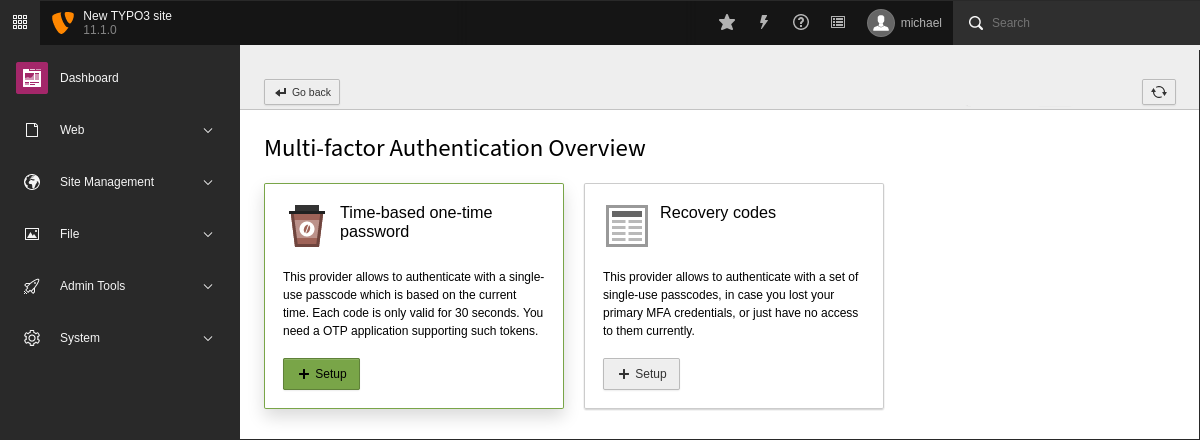
\includegraphics[width=0.8\linewidth]{ChangesForIntegratorsAndDevelopers/1613731375-MultiFactorAuthentication.png}
	\end{figure}

\end{frame}

% ------------------------------------------------------------------------------

% ------------------------------------------------------------------------------
% TYPO3 Version 11.1 - What's New (English Version)
%
% @author	Michael Schams <schams.net>
% @license	Creative Commons BY-NC-SA 3.0
% @link		http://typo3.org/download/release-notes/whats-new/
% @language	English
% ------------------------------------------------------------------------------
% Feature | 93526 | Multi-Factor Authentication (2)

\begin{frame}[fragile]
	\frametitle{Changes for Integrators and Developers}
	\framesubtitle{Multi-Factor Authentication (2)}

	\lstset{basicstyle=\fontsize{6}{8}\ttfamily}

	\begin{itemize}
		\item ...
	\end{itemize}

\end{frame}

% ------------------------------------------------------------------------------


% Chapter "Extbase and Fluid"
% ------------------------------------------------------------------------------
% TYPO3 Version 11.1 - What's New (Italian Version)
%
% @license	Creative Commons BY-NC-SA 3.0
% @link		http://typo3.org/download/release-notes/whats-new/
% @language	Italian
% ------------------------------------------------------------------------------

\section{Extbase and Fluid}
\begin{frame}[fragile]
	\frametitle{Extbase and Fluid}

	\begin{center}\huge{Chapter 3:}\end{center}
	\begin{center}\huge{\color{typo3darkgrey}\textbf{Extbase and Fluid}}\end{center}

\end{frame}

% ------------------------------------------------------------------------------

% ------------------------------------------------------------------------------
% TYPO3 Version 11.1 - What's New (English Version)
%
% @author	Michael Schams <schams.net>
% @license	Creative Commons BY-NC-SA 3.0
% @link		http://typo3.org/download/release-notes/whats-new/
% @language	English
% ------------------------------------------------------------------------------
% Feature | 92338 | Allow link text wrapping in TypolinkViewhelper

\begin{frame}[fragile]
	\frametitle{Extbase and Fluid}
	\framesubtitle{TypolinkViewhelper}

	\lstset{basicstyle=\fontsize{6}{8}\ttfamily}

	\begin{itemize}
		\item The ViewHelper \texttt{f:link.typolink} features a new argument
			\texttt{textWrap} which wraps the link title.

		\item For example:
\begin{lstlisting}
<f:link.typolink parameter="123" textWrap="<span>|</span>" />
\end{lstlisting}

		\item Output:
\begin{lstlisting}
<a href="page-123"><span>My page title</span></a>
\end{lstlisting}

		\item Note: don't forget to scape quotes:
\begin{lstlisting}
<f:link.typolink parameter="123" textWrap="<span class=\"small\">|</span>" />
\end{lstlisting}

	\end{itemize}

\end{frame}

% ------------------------------------------------------------------------------


% Chapter "Deprecated and Removed Functions"
% ------------------------------------------------------------------------------
% TYPO3 Version 11.1 - What's New (Italian Version)
%
% @license	Creative Commons BY-NC-SA 3.0
% @link		http://typo3.org/download/release-notes/whats-new/
% @language	Italian
% ------------------------------------------------------------------------------

\section{Extbase and Fluid}
\begin{frame}[fragile]
	\frametitle{Extbase and Fluid}

	\begin{center}\huge{Chapter 3:}\end{center}
	\begin{center}\huge{\color{typo3darkgrey}\textbf{Extbase and Fluid}}\end{center}

\end{frame}

% ------------------------------------------------------------------------------

% ------------------------------------------------------------------------------
% TYPO3 Version 11.1 - What's New (English Version)
%
% @author	Michael Schams <schams.net>
% @license	Creative Commons BY-NC-SA 3.0
% @link		http://typo3.org/download/release-notes/whats-new/
% @language	English
% ------------------------------------------------------------------------------
% Deprecation | 93149 | T3Editor JavaScript module replaced by CodeMirrorElement

\begin{frame}[fragile]
	\frametitle{Deprecated/Removed Functions}
	\framesubtitle{T3editor}

	\lstset{basicstyle=\fontsize{6}{8}\ttfamily}

	\begin{itemize}
		\item The T3Editor has been refactored into a custom HTML element:
\begin{lstlisting}
<typo3-t3editor-codemirror>
\end{lstlisting}

		\item The element features a new JavaScript module:\newline
			\small
				\texttt{TYPO3\textbackslash
					CMS\textbackslash
					T3editor\textbackslash
					Element\textbackslash
					CodeMirrorElement}
			\normalsize

		\item Using the CSS class "\texttt{t3editor}" is now \textbf{deprecated}:
\begin{lstlisting}
<textarea class="t3editor"> ... </textarea>
\end{lstlisting}

	\end{itemize}

\end{frame}

% ------------------------------------------------------------------------------

% ------------------------------------------------------------------------------
% TYPO3 Version 11.1 - What's New (German Version)
%
% @license	Creative Commons BY-NC-SA 3.0
% @link		http://typo3.org/download/release-notes/whats-new/
% @language	German
% ------------------------------------------------------------------------------
% Deprecation | 93454 | Rename Sortable to sortablejs

\begin{frame}[fragile]
	\frametitle{Veraltete/Entfernte Funktionen}
	\framesubtitle{SortableJS}

	\begin{itemize}
		\item Die JavaScript-Bibliothek \texttt{SortableJS} wurde auf \texttt{sortablejs} umbenannt.

		\item Diese Änderung war aufgrund des Imports von TypeScript-Deklarationen 
			von \texttt{SortableJS} erforderlich.

		\item Der bisherige Name \texttt{Sortable} wurde als \textbf{veraltet} markiert.

		\item Erweiterungsentwicklern wird empfohlen, die Bibliothek mit ihrem neuen Namen zu verwenden.
	\end{itemize}

\end{frame}

% ------------------------------------------------------------------------------

% ------------------------------------------------------------------------------
% TYPO3 Version 11.1 - What's New (German Version)
%
% @license	Creative Commons BY-NC-SA 3.0
% @link		http://typo3.org/download/release-notes/whats-new/
% @language	German
% ------------------------------------------------------------------------------
% Deprecation | 93506 | jQuery in tooltips

\begin{frame}[fragile]
	\frametitle{Veraltete/Entfernte Funktionen}
	\framesubtitle{jQuery in Tooltips}

	\lstset{basicstyle=\fontsize{6}{8}\ttfamily}

	\begin{itemize}
		\item Die Übergabe von jQuery-Objekten an die Methoden \texttt{show()} und \texttt{hide()}
			des Moduls \texttt{TYPO3/CMS/Backend/Tooltip} wurde als
			\textbf{veraltet} markiert.
		\item Dies führt zu einer Deprecation-Warnung in der Konsole des Browsers.
		\item Migrationsmöglichkeiten:
			Ein einzelnes\texttt{HTMLElement} oder eine \texttt{NodeList} and die
			Funktionen übermitteln.
	\end{itemize}

\end{frame}

% ------------------------------------------------------------------------------


% Chapter "Sources and Authors"
% ------------------------------------------------------------------------------
% TYPO3 Version 11.1 - What's New (Italian Version)
%
% @license	Creative Commons BY-NC-SA 3.0
% @link		http://typo3.org/download/release-notes/whats-new/
% @language	Italian
% ------------------------------------------------------------------------------

\section{Extbase and Fluid}
\begin{frame}[fragile]
	\frametitle{Extbase and Fluid}

	\begin{center}\huge{Chapter 3:}\end{center}
	\begin{center}\huge{\color{typo3darkgrey}\textbf{Extbase and Fluid}}\end{center}

\end{frame}

% ------------------------------------------------------------------------------

% ------------------------------------------------------------------------------
% TYPO3 Version 11.1 - What's New (German Version)
%
% @license	Creative Commons BY-NC-SA 3.0
% @link		http://typo3.org/download/release-notes/whats-new/
% @language	German
% ------------------------------------------------------------------------------
% Sources

\begin{frame}[fragile]
	\frametitle{Quellen und Autoren}
	\framesubtitle{Quellen}

	\textbf{TYPO3 News:}
		\begin{itemize}\smaller
			\item \url{https://typo3.org/project/news/}
		\end{itemize}

	\textbf{Release Infos:}
		\begin{itemize}\smaller
			\item \url{https://get.typo3.org/release-notes/11.x/TYPO3_CMS_11.1.0}
			\item \href{https://docs.typo3.org/c/typo3/cms-core/master/en-us/Changelog-11.html}{TYPO3 v11 ChangeLog}
			\item \texttt{typo3/sysext/core/Documentation/Changelog/11.1/*}
		\end{itemize}

	\textbf{TYPO3 Bug-/Issuetracker:}
		\begin{itemize}\smaller
			\item \url{https://forge.typo3.org/projects/typo3cms-core}
		\end{itemize}

	\textbf{TYPO3 und Fluid Git Repositories:}
		\begin{itemize}\smaller
			\item \url{https://git.typo3.org/Packages/TYPO3.CMS.git}
			\item \url{https://github.com/TYPO3/Fluid}
		\end{itemize}

\end{frame}

% ------------------------------------------------------------------------------

% ------------------------------------------------------------------------------
% TYPO3 Version 11.1 - What's New (French Version)
%
% @license	Creative Commons BY-NC-SA 3.0
% @link		http://typo3.org/download/release-notes/whats-new/
% @language	French
% ------------------------------------------------------------------------------
% The TYPO3 CMS What's New Team

\begin{frame}[fragile]
	\frametitle{Sources et Auteurs}

	\vspace{-0.6cm}

	\centerline{\textbf{Équipe TYPO3 CMS What's New~:}}

	\begin{center}
		\centerline{Pierrick Caillon, Richard Haeser, Jigal van Hemert,}
		\centerline{Henrietta Kucsovan, Corina Miron, Sinisa Mitrovic,}
		\centerline{Michael Schams, and Roberto Torresani}
	\end{center}

	\vspace{0.6cm}

	\smaller\begin{center}\url{https://typo3.org/help/documentation/whats-new/}\end{center}\normalsize

	\vspace{1cm}

	\smaller\begin{center}Sous license Creative Commons BY-NC-SA 3.0\end{center}\normalsize
	\begin{figure}\vspace*{-0.4cm}
		
\includegraphics[width=1.4cm]{SourcesAndAuthors/CreativeCommons-BY-NC-SA.png}
	\end{figure}

\end{frame}

% ------------------------------------------------------------------------------


% ------------------------------------------------------------------------------
\end{document}
